\documentclass[pdftex,cyrillic,14pt,a4page,twoside]{extreport}
\usepackage[bulgarian]{babel}

\usepackage[margin=2cm]{geometry}% http://ctan.org/pkg/geometry
\usepackage[pdftex]{graphicx}
\graphicspath{ {./figures/} }

\usepackage{./titlesec/titlesec}

% Counter too wide line spacing added by twoside
% https://tex.stackexchange.com/questions/62572/twoside-introduces-incorrect-linespacing-at-end-of-section
\raggedbottom
  
\titleformat{\chapter}%
  {\normalfont\bfseries\Huge}{\thechapter.}{10pt}{}

\usepackage{afterpage}
\newcommand\blankpage{%
    \null
    \thispagestyle{empty}%
    \newpage}


\begin{document}
\begin{titlepage}
	\begin{center}
	
\includegraphics[scale=1.2]{./NBU_logo.jpg}\\[0.3cm]
    \textbf{\Large НОВ БЪЛГАРСКИ УНИВЕРСИТЕТ\\[0.4cm]}
    \textbf{\Large Департамент Информатика\\[0.4cm]}
    \textbf{\Large Бакалавърка програма Информатика\\[3cm]}
   
		\textbf{\LARGE Автоматизиран биоинформатичен анализ на генетични варианти, потенциално свързани със стареенето\\[2cm]}
		\begin{Large}
		Дипломна работа на\\[0.2cm]
		Михаил М. Здравков\\[3cm]
		\end{Large}
		\begin{minipage}{0.48\textwidth}
			\begin{flushleft} \large
				\emph{Научни ръководители:} \\
				доц. д-р Милена Георгиева \\
				Момчил Топалов
			\end{flushleft}
		\end{minipage}
			\begin{minipage}{0.48\textwidth}
			\begin{flushright} \large
				\emph{Ръководител катедра:} \\
				гл. ас. д-р Методи Трайков\\
				\clearpage
			\end{flushright}
		\end{minipage}

		\vfill

		% Bottom of the page
		{\large София 2022}

	\end{center}
\end{titlepage}


\afterpage{\blankpage}

\newgeometry{
	inner=30mm,
    outer=20mm,
    top=20mm,
    bottom=20mm}

\tableofcontents
\pagebreak
\afterpage{\blankpage}

\setlength\parindent{0pt}

\chapter{Увод}
\paragraph{}

Стареенето е естествен процес, който има огромно значение както за отделния индивид, така и за обществото като цяло. С напредването на възрастта, рискът от разнообразни заболявания като рак, болест на Алцхаймер, диабет, сърдечно-съдови заболявания и др. нараства значително. Смята се, че около две-трети от смъртните случаи при хора се дължат на заболявания, свързани с възрастта. Същевременно, с глобалното нарастване на средната продължителност на живота, проблемите на стареенето засягат все повече хора и имат все по-голямо обществено значение. От социална гледна точка, стареенето оказва значителен икономически и демографски ефект.

\paragraph{}
Установено е, че процесът на стареене се влияе както от генетични, така и от епигенетични фактори. Въпреки това, този процес все още не е достатъчно добре разбран от науката, поради което е трудно да се създадат ефективни методи за терапия и справяне с негативните му ефекти.

\paragraph{}
Настоящата дипломна работа се фокусира върху генетичната основа на стареенето. Основен подход при нейното изследване е анализът на генетични варианти. При такива изследвания е необходима обработката на големи обеми от данни, което налага нуждата от използване на специализиран биоинформатичен софтуер. Налични са множество различни инструменти, покриващи различни аспекти от обработката на файлове с генетични варианти - анотация, филтриране, анализ и тн. Повечето от тях, обаче, изискват значителни технически познания, което ги прави трудни за използване от специалисти в други области, като биология и генетика.

\paragraph{}
Целта на настоящата дипломна работа е създаването на интегрирана софтуерна система за биоинформатични изследвания на генетични варианти и предсказване на тяхната потенциална асоциация с процеса на стареене. Надяваме се, чрез създаване на по-достъпен инструмент, да допринесем за бъдещи изследвания на процеса на стареене и за търсенето на ефективни терапии против негативните му ефекти.
            
\chapter{Литературен обзор}
\section{Значение на стареенето}
\subsection{Дефиниция}
\paragraph{}
Въпреки, че концепцията за стареене е универсално разбираема, формалната ѝ дефиниция не е тривиална и множество автори дават твърде различни определения за този термин. Аркинг (2006, стр. 11) прави преглед на наличната литература и, в резултат, предлага следната дефиниция\cite{arking2006biology}:

\paragraph{}
\textit{„Стареенето е независима от времето поредица от кумулативни, прогресивни, свойствени и вредящи структурни и функционални промени, които обикновено започват да се изразяват при репродуктивната зрялост и приключват със смъртта.“}

\paragraph{}
Макар времето да няма каузална връзка с ефектите на стареенето, то корелацията помежду им е причина обикновено да се говори за ефектите на стареенето като за нещо, настъпващо с напредването на възрастта.

\subsection{Физиологични ефекти}
\paragraph{}
Стареенето оказва изключително голям ефект върху човешкото тяло. То обикновено включва широк спектър от различни физиологични промени, които влошават жизнеността и качеството на живот на индивида. Примери за това са понижена фертилност при жените\cite{kamath2010}; загуба на телесна маса\cite{spencer1996}; влошен слух\cite{feder2015}; повишен риск от хронични заболявания\cite{larson2013}\cite{prasad2012}; хронична болка\cite{geriatrics2002}; загуба на сила и еластичност в мускулно-скелетната система; понижената способност за устояване на инфекции, екстремни температури и др. видове стрес; влошаване на зрението; загуба на неврологични функции\cite{vina2007} и др.


\subsection{Демографски и икономически ефекти}
\paragraph{}
През последния един век очакваната продължителност на живота в целия свят драстично се е повишила\cite{zijdeman2016} (виж фиг. \ref{fig:life_expectancy}). Освен безспорните ползи, това води и до редица проблеми. Удължаването на продължителността на живота, в комбинация с наблюдавания спад на раждаемостта, се очаква да доведе до застаряване на населението\cite{lutz2008}. Световната Здравна Организация (СЗО) предупреждава, че се очаква между 2015 и 2050 броят на хората над 60-годишна възраст да се повиши от 12\% от населението до 22\%\cite{who_report_ageing2015}. Същевременно, по данни на СЗО, увеличаването на продължителността на живота (с 6 години за периода между 2000 и 2019) изпреварва увеличаването в продължителността на здравословния живот (с 5.4 години за същия период)\cite{who_health2020}. \\
\begin{figure}[h]
  \centering
  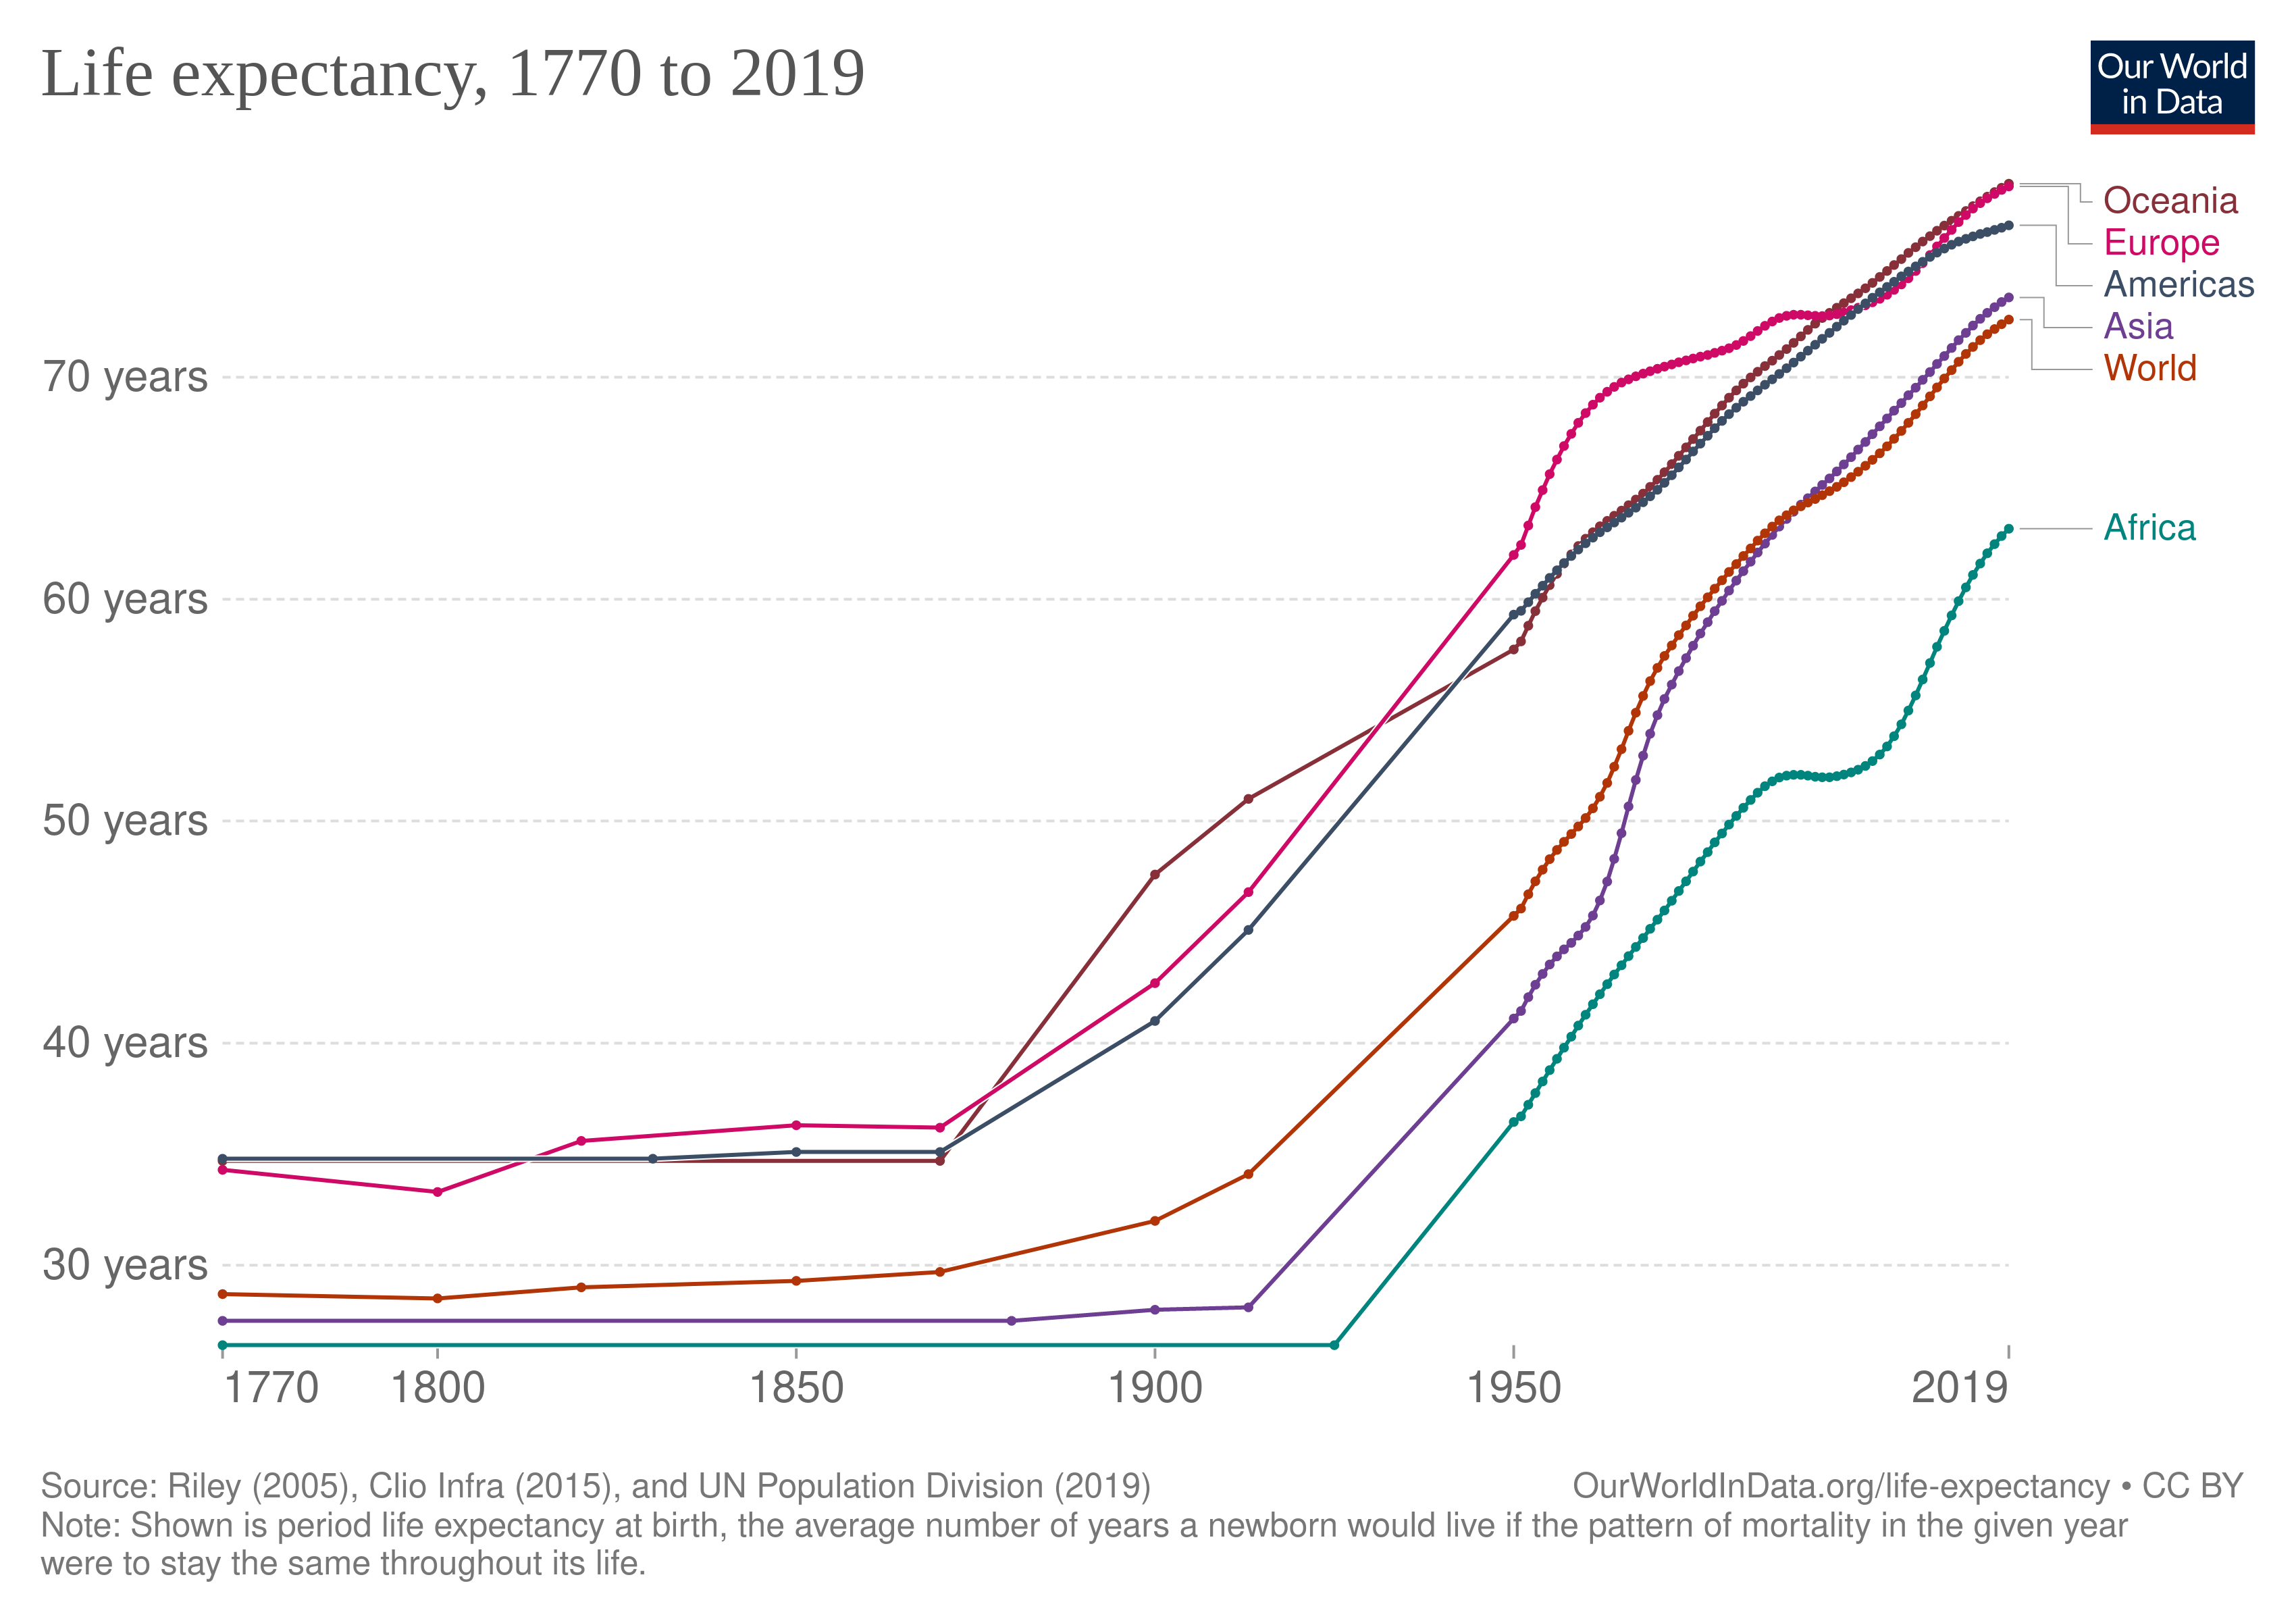
\includegraphics[width=12cm]{figures/life-expectancy}
  \caption {Очаквана продължителност на живота за различни региони}
  \label{fig:life_expectancy}
\end{figure}

\paragraph{}
Застаряването на населението би оказало неблагоприятен ефект и върху икономиката на държавите. Първо, заради увеличаването на дяла на хора, които не участват в работната сила. Второ, поради това, че здравните системи ще бъдат допълнително натоварени с по-голям брой хора в напреднала възраст, за които рисковете от хронични заболявания са значително по-големи.


\section{Молекулярно-биологични теории\\ за стареенето}
\paragraph{}
Стареенето е въпрос, който вълнува учените от дълго време. През 1990-та, Медведев твърди, че вече съществуват над 300 теории за стареенето\cite{medvedev1990}. Въпреки постигнатият значителен прогрес през последните години в областта на геронтологията, причините за стареенето все още оставан ненапълно обяснени. Това се дължи на факта, че стареенето е сложен процес, в който са намесени множество фактори. Все още липсва голяма обединяваща теория на стареенето, която да обясни изцяло процеса, но съществуват множество теории, които дават добра представа за различни негови аспекти\cite{vina2007}. Следва кратък преглед на основните теории:

\subsection{Натрупване на геномни изменения}
\paragraph{}
Изменения в ДНК молекулите могат да настъпят както в следствие на вътрешноклетъчни фактори, така и поради въздействието на външни мутагени. Примери за вътрешноклетъчни фактори са случайни грешки при репликация и оксидативния стрес, предизвикан от натрупването на свободни радикали\cite{wang1998}. Външните мутагени могат да бъдат разделени на три вида - физични, химични и биологични. Пример за физичен мутаген е радиацията\cite{breimer1988}, a за биологичен вирусните инфекции, които също могат да предизвикат генетични мутации. Измененията в ДНК молекулите включват различни видове мутации като точкови мутации, делеции и инсерции, транслокации, инверсии и др.\\\\
Съществуват механизми, чрез които клетките засичат мутациите и ги поправят. Основни такива механизми са гените ATM и TP53. Все пак, тези механизми не са ефективни на 100\% и ефективността им допълнително спада с възрастта\cite{auley2017}. В резултат, в течение на времето, ДНК молекулите акумулират все повече мутации. Смята се, че тази геномна нестабилност е един от основните фактори, допринасящи за процеса на стареенето\cite{vijg2013}.

\subsection{Скъсяване на теломерите}
\paragraph{}
Теломерите са регион, намиращ се в края на хромозомите, в който се съдържат повтарящи се поредици от нуклеотидни бази. Те служат за предпазване на хромозомата от рекомбинация и постепенна деградация и дават възможност на клетката да различава края на хромозомата от случайни прекъсвания, при които биха били активирани механизмите за поправка на ДНК\cite{griffith1999}. При всеки цикъл на делене на клетката, теломерите се скъсяват поради непълното синтезиране на изоставащата нишка от ДНК полимеразата\cite{koliada2015}. Този проблем се компенсира донякъде от ензима теломераза, който пренася своя собствена РНК молекула и я използва като шаблон, спрямо който да удължи скъсения теломер. Въпреки това, недостатъчната експресия на теломеразата води до постепенното скъсяване на теломерите. Това може да доведе до загуба на репликативна способност на клетката и блокирането на клетъчния ѝ цикъл, процес известен като клетъчно стареене\cite{muraki2012}.

\subsection{Клетъчно стареене}
TODO

\subsection{Епигенетични изменения}
TODO

\chapter{Генетични фактори,\\ влияещи на процеса\\ на стареене}
\paragraph{}
В секция 2.2 беше представен кратък обзор на различните биологични процеси, които способстват процеса на стареене. Уместен е въпросът дали има определени генетични фактори, които оказват въздействие на тези процеси. Ако това е така, бихме могли да очакваме, че съществуват генни алели, които забързват или забавят стареенето. В текущата глава ще разгледаме въпроса за съществуването на такива генни алели, както и за начините им на действие и методите за изследването им. 

\section{Съществуване}
\paragraph{}


\section{Начин на действие}
\section{Проблеми на изследването им}
\chapter{Обзор на съществуващи\\ биоинформатични решения}
\section{Анотация}
\subsection{snpEff}
\subsection{VEP}
\subsection{Annovar}
\section{Филтриране и анализ на генетични\\ варианти}
\subsection{snpSift}
\subsection{???}
\section{Геномни браузъри}
\subsection{UCSC Genome Browser}
\subsection{IGV Genome Browser}
\section{Нагъване на протеини}
\subsection{Подходи}
\subsection{AlphaFold}
\section{Интегрирани софтуерни решения}
\subsection{Galaxy Project}
\chapter{Цели}
\chapter{Задачи}
\chapter{Представяне на\\ софтуерното решение}
\section{Софтуерна архитектура}
\section{Структура на базата данни}
\section{Управление на генни множества}
\section{Обработка на VCF при импортиране}
\section{Операции върху импортиран VCF}
\chapter{Дискусия}
\chapter{Изводи}
\chapter*{Използвани външни\\ библиотеки и софтуер}
\addcontentsline{toc}{chapter}{Използвани външни библиотеки и софтуер}

%\chapter*{Използвана литература}
%\addcontentsline{toc}{chapter}{Използвана литература}

\bibliographystyle{plain}
\bibliography{refs}
\addcontentsline{toc}{chapter}{Библиография}

\end{document}